\documentclass[tikz,border=4pt]{standalone}
\usepackage{amsmath}
\begin{document}
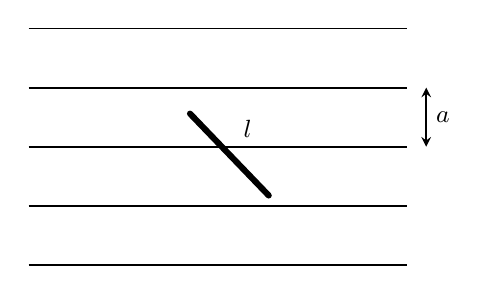
\begin{tikzpicture}[>=stealth, thick, scale=1.0]
  % Five parallel horizontal lines spaced by a = 0.75 cm
  \foreach \y in {0, 0.75, 1.50, 2.25, 3.00} {
    \draw[line width=0.65pt] (-2.4, \y) -- (2.4, \y);
  }
  % Spacing label a
  \draw[<->, line width=0.55pt] (2.65, 1.50) -- (2.65, 2.25) node[midway, right, font=\small] {$a$};

  % Dropped needle of length l >= a (here l ~ 1.45 cm > 0.75 cm)
  \draw[line width=2.2pt, line cap=round] (-0.35, 1.92) -- (0.65, 0.88);
  \node[above right, font=\small] at (0.20, 1.48) {$l$};
\end{tikzpicture}
\end{document}
